%lezione 17 del 22 aprile 2026 pag 38 appunti
%-----------------------------------------------------------------------------------------------------
\newpage
%\addtocontents{toc}{\protect\newpage}
\chapter{Scattering}\\

In questa parte del corso si tratterà la teoria dello scattering elastico quantistico, che viene
studiato confrontando lo stato della particella "proiettile" prima e dopo aver interagito con un
bersaglio: gli stati iniziale e finale sono entrambi di particella libera con impulso dello stesso
modulo, ma con direzioni diverse.
\section{Concetti e definizioni generali}
Si considerano urti in 3 dimensioni e il sistema di riferimento è tale da avere l'asse $z$ parallelo
al momento della particella incidente $\mathbf{p}$: si utilizzano le coordinate sferiche riferite a
tale asse, come illustrato in figura \ref{fig:scattering}.
\begin{figure}[H]
    \centering
    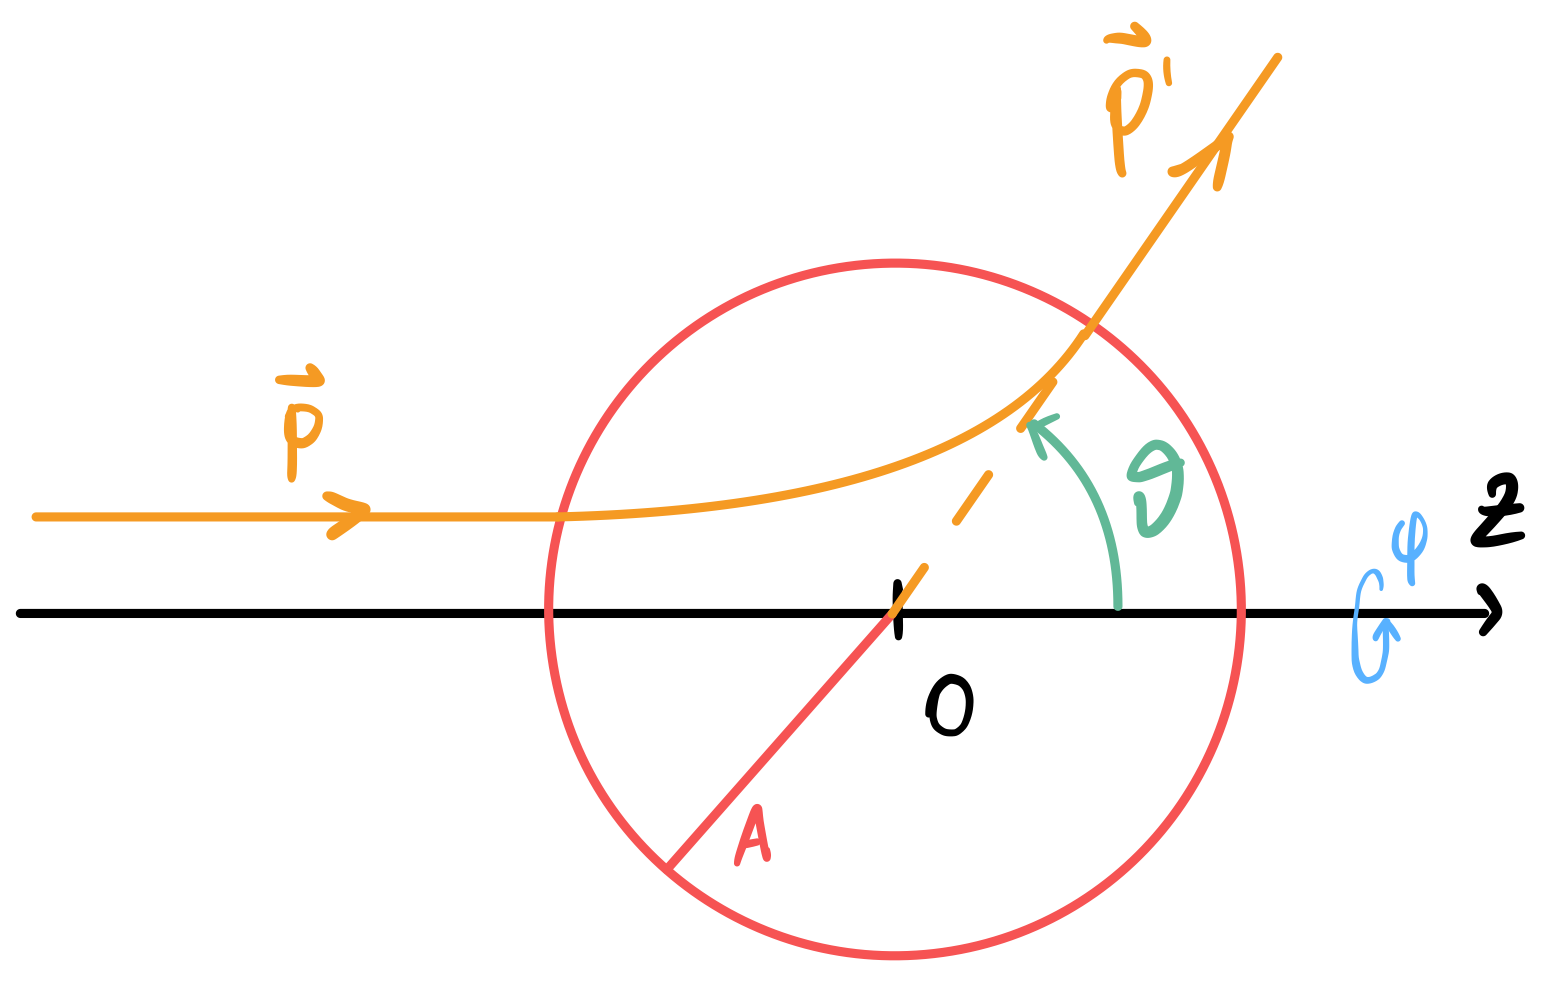
\includegraphics[width = 0.65\linewidth]{./figures/scattering.png}
    \caption{\small Schema dello scattering elastico con un potenziale a range finito.}
    \label{fig:scattering}
\end{figure}
In questa trattazione non si considereranno né effetti relativistici né urti anelastici e si
supporrà che non avvengano mai né scattering multiplo (approssimazione di bersaglio sottile), né
effetti di interferenza tra particelle che colpiscono bersagli diversi ($\lambda_{DeB}<<\text{distanza
tra bersagli}$).
\subsection{Sezione d'urto}
Il flusso di particelle incidenti è definito come 
$$F_i = \frac{\text{n. ptc.}}{tA}$$
dove $t$ è il tempo e $A$ è la sezione del fascio.\\
Si consideri ora una porzione infinitesima di angolo solido $d\Omega$ attorno alla direzione
generica $\vartheta$: il rate di particelle osservate in un "intorno" $d\Omega$ di $\vartheta$ è
$dn=\dv[]{n}{\Omega}d\Omega$ e, poiché il rate uscente dipende dal flusso entrante, si definisce la
\textbf{sezione d'urto differenziale}:
$$\sigma(\vartheta,\varphi) = \dv[]{\sigma}{\Omega}:=\dv[]{n}{\Omega}\frac{1}{F_i}$$
che ha le dimensioni di un'area e si misura in Barn ($1\text{b}=10^{-24}$cm$^2$): può essere
interpretata geometricamente come la parte di area del fascio incidente che produce il fascio uscente
ad angolo $\vartheta$.

Si definisce inoltre la \textbf{sezione d'urto totale}:
$$\sigma_\text{tot} = \int d\Omega \dv[]{\sigma}{\Omega}$$
\subsection{Bersaglio e potenziale}
Nella maggioranza dei casi, il potenziale di interazione dipende solo dalla distanza tra le particelle
interagenti: dette $\mathbf{r_1},\mathbf{r_2}$ le coordinate del proiettile e del bersaglio, si ha
$$V(\mathbf{r_1},\mathbf{r_2}) = V(\mathbf{r_1}-\mathbf{r_2})$$
per questa tipologia di potenziali si può fattorizzare l'Hamiltoniana del sistema definendo le
quantità
$$\begin{dcases}
    \mathbf{R} = \frac{m_1\mathbf{r_1}+m_2\mathbf{r_2}}{m_1+m_2}\\
    \mathbf{r} = \mathbf{r_1}-\mathbf{r_2}\\
    M = m_1+m_2\\
    \mu = \frac{m_1m_2}{m_1+m_2}
\end{dcases}$$
l'Hamiltoniana risulta dunque
$$H = T_1 + T_2 + V = H_{cm} + H_r$$
con
$$
\begin{dcases}
    H_{cm} = \frac{\mathbf{P}^2}{2M}&\text{Hamiltoniana del centro di massa}\\
    H_r = \frac{\mathbf{p}^2}{2\mu} + V(\mathbf{r})&\text{Hamiltoniana di una particella in un
    potenziale}
\end{dcases}
$$
dove si è chiamato $\mathbf{P}$ il momento del centro di massa del sistema.\\
Come in meccanica classica, questa fattorizzazione permette di ignorare il moto complessivo del
sistema e di ridurre l'interazione tra due corpi al moto di uno solo in un potenziale diverso.

L'altra ipotesi che si fa sul potenziale è che esso sia a corto raggio, cioè che $\exists A$ tale che
$V(\mathbf{r})\approx0$ per $|\mathbf{r}|>A$.
\section{Risoluzione dell'equazione di Schrödinger}
Si cercano le soluzioni stazionarie con $E\in Spc(H)$ del problema con equazione
$$-\frac{\hbar^2}{2\mu}\laplacian\psi(\mathbf{x})+V(\mathbf{x})\psi(\mathbf{x})=E\psi(\mathbf{x})
\rightarrow\left(\laplacian + k^2\right)\psi(\mathbf{x})=U(\mathbf{x})\psi(\mathbf{x})$$
dove si sono definiti
$$k^2 = \frac{2mE}{\hbar^2}\text{,}\phantom{x}U(\mathbf{x})=\frac{2m}{\hbar^2}V(\mathbf{x})$$

Si cercano soluzioni $\psi(\mathbf{x})$ tali che a $t=0$ e $z=-\infty$ siano onde piane con numero
d'onda $\mathbf{k}=\frac{1}{\hbar}\mathbf{p}$ e che per $t\to\infty$ tornino ad essere onde piane
con $\mathbf{k'}$ tale che $|\mathbf{k'}|=|\mathbf{k}|$.
\subsection{Determinazione della funzione di Green}
Per risolvere l'equazione di Schrödinger, si cerca la funzione di Green $G(\mathbf{x},\mathbf{y})$
tale che
$$\left(\laplacian + k^2\right)G(\mathbf{x},\mathbf{y}) = \delta^3(\mathbf{x}-\mathbf{y})$$
La soluzione, in forma integale, sarà
$$\psi(\mathbf{x}) = \psi_\text{hom}(\mathbf{x}) +
\int_{}^{}d^3\mathbf{y}G(\mathbf{x},\mathbf{y})U(\mathbf{y})\psi(\mathbf{y})$$
dove $\psi_\text{hom} = Ae^{i\mathbf{k}\cdot\mathbf{x}}$ è la soluzione dell'equazione omogenea
(che è quella di una particella libera).
\newpage
Si cerca una $G$ che abbia le stesse simmetrie dell'operatore $\laplacian + k^2$:
\begin{itemize}
    \item Invarianza per traslazione: $G(\mathbf{x},\mathbf{y})=G(\mathbf{x+a},\mathbf{y+a})$,
	si può dunque porre $\mathbf{y}=0$ e $G=G(\mathbf{x})$;
    \item Invarianza per rotazione: $G(\mathbf{x})=G(|\mathbf{x}|):=G(r)$.
\end{itemize}
Si impone ora la definizione di $G$ per trovarla:
$$(\laplacian + k^2)G(r) = \delta^3(\mathbf{x})\rightarrow
\frac{1}{r}\dv[2]{}{r}\left(rG(r)\right)+k^2G(r)=\delta^3(\mathbf{x})$$
dove si è riscritto il $\laplacian$ in coordinate sferiche, ignorando la parte angolare.

Per $r\not=0$, la $\delta^3$ si annulla e si ha, per somiglianza con l'equazione armonica:
$$\dv[2]{}{r} \left(rG(r)\right)+k^2rG(r)=0 \to rG(r)=Ae^{\pm ikr} \to G(r)= A\frac{e^{\pm ikr}}{r}$$
dove $A$ è una costante da determinare.
